\documentclass[12pt]{article}
\usepackage{amsmath}
\usepackage{amssymb}
\usepackage{geometry}
\usepackage{enumerate}
\usepackage{natbib}
\usepackage{float}%稳定图片位置
\usepackage{graphicx}%画图
\usepackage[english]{babel}
\usepackage{a4wide}
\usepackage{indentfirst}%缩进
\usepackage{enumerate}%加序号
\usepackage{multirow}%合并行
\title{\large UM-SJTU JOINT INSTITUTE\\Advanced Lasers and Optics Laboratory\\(VE438)\\\ \\\ \\\ \\\ \\\ \\\ \\\ \\\ \\\ \\\ \\\
Post Lab Assignment\\\ \\\ LAB 1\\\ Polarization, Total Internal
Reflection and Single Slit Diffraction \\\ \\\ \\\ \\\ \\\ }
\author{Name: Pan Chongdan \\ID: 516370910121}
\date{Date: \today}

\begin{document}
\maketitle
\newpage

\section{PART A: Polarization}
\subsection{Measurement data}
\begin{table}[H]
\centering
\begin{tabular}{|c|c|c||c|c|c|}
\hline
rotation angle $\theta$    &measured voltage $mV$&rotation angle $\theta$    &measured voltage $mV$   \\ \hline
$0^o$       &369.4     &$90^o$      &5.3     \\ \hline
$5^o$      	&368.7     &$95^o$      &67.7     \\ \hline
$10^o$      &367.6     &$100^o$     &150.3     \\ \hline
$15^o$      &364.4     &$105^o$     &205.4     \\ \hline
$20^o$      &359       &$110^o$     &239.5     \\ \hline
$25^o$      &355.1     &$115^o$     &267.0     \\ \hline
$30^o$      &354       &$120^o$     &286.6     \\ \hline
$35^o$      &351.9     &$125^o$     &301.9     \\ \hline
$40^o$      &342.7     &$130^o$     &316.1     \\ \hline
$45^o$      &333.0     &$135^o$     &327.0     \\ \hline
$50^o$      &318.4     &$140^o$     &334.0     \\ \hline
$55^o$      &304.2     &$145^o$     &347.4     \\ \hline
$60^o$      &286.5     &$150^o$     &352.0     \\ \hline
$65^o$      &264.4     &$155^o$     &357.5     \\ \hline
$70^o$      &239.6     &$160^o$     &362.2     \\ \hline
$75^o$      &196       &$165^o$     &365     \\ \hline
$80^o$      &147.4     &$170^o$     &366.1     \\ \hline
$85^o$      &66.8      &$175^o$     &369.0     \\ \hline
\end{tabular}
\end{table}
\begin{figure}[H]
\centering
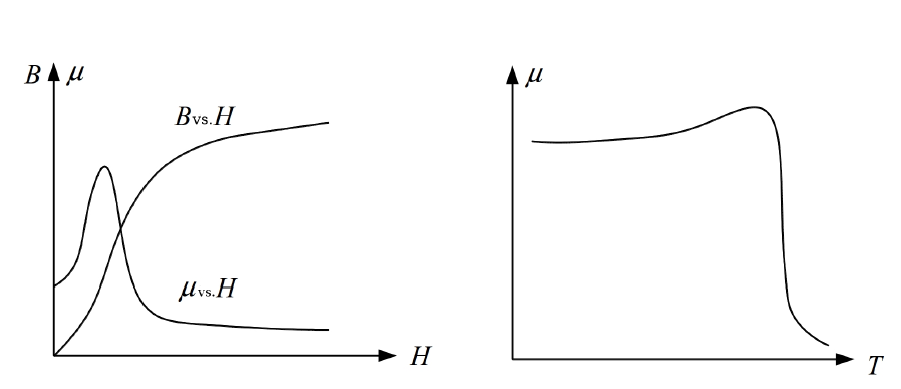
\includegraphics[scale=0.5]{P1.jpg}
\caption{Relation between voltage (light intensity) and rotation angle}
\end{figure}
\subsection{Answers for Post Lab Questions}
Since the emitted light is linear polarized light, so it won't change much when we set the polarizer to zero point but after we start to rotated the polarizer, the light becomes darker and we're hardly to see the light after we rotated if for 90 degrees. Then the light come back during subsequent rotation. So the light intensity first become smaller than it grown back when we rotated the polarizer. The relation between the intensity and rotation angle is like the plot.
\par However, even when the rotation is 90 degree and the light intensity is very small, there was still some reading ,which means the laser been can't be totally blocked.
\par According to Malus's Law, $I_{light}=I_{light,0}\cos ^2\theta$, where $\theta$ is the angle between the angle of polarizer and the direction of the polarization of the light. Since the $I_light$ can't be 0, then $\cos^2\theta$ can't be $90^o$ ,so the emitted light is not totally linear polarized.
\section{PART B: Total Internal Reflection}
\subsection{Measured Data}
We find critical angle for the total internal reflection when the incident angle is $219.5^o-180^o=39.5^o$. So the critical angle is also $39.5^o$. Since $$\frac{\sin\theta_i}{\sin\theta_o}=\frac{n_i}{n_o}$$ and $\sin\theta_o=1,n_i=1$, then
$n_o=\frac{1}{\sin39.5}=1.57$
\par So the refractive index of the prism is 1.57
\subsection{Answers for Post Lab Questions}
First, we put the prism at the center of rotation stage so that the incident light was perpendicular to the long edge of the prism. Then we started to rotate the rotation stage until the refracted light was parallel to the long edge of the prism, which means the refraction angle is $90^o$. At the time, the angle we rotated is also the incident angle, which is both $39.5^o$
\begin{figure}[H]
\centering
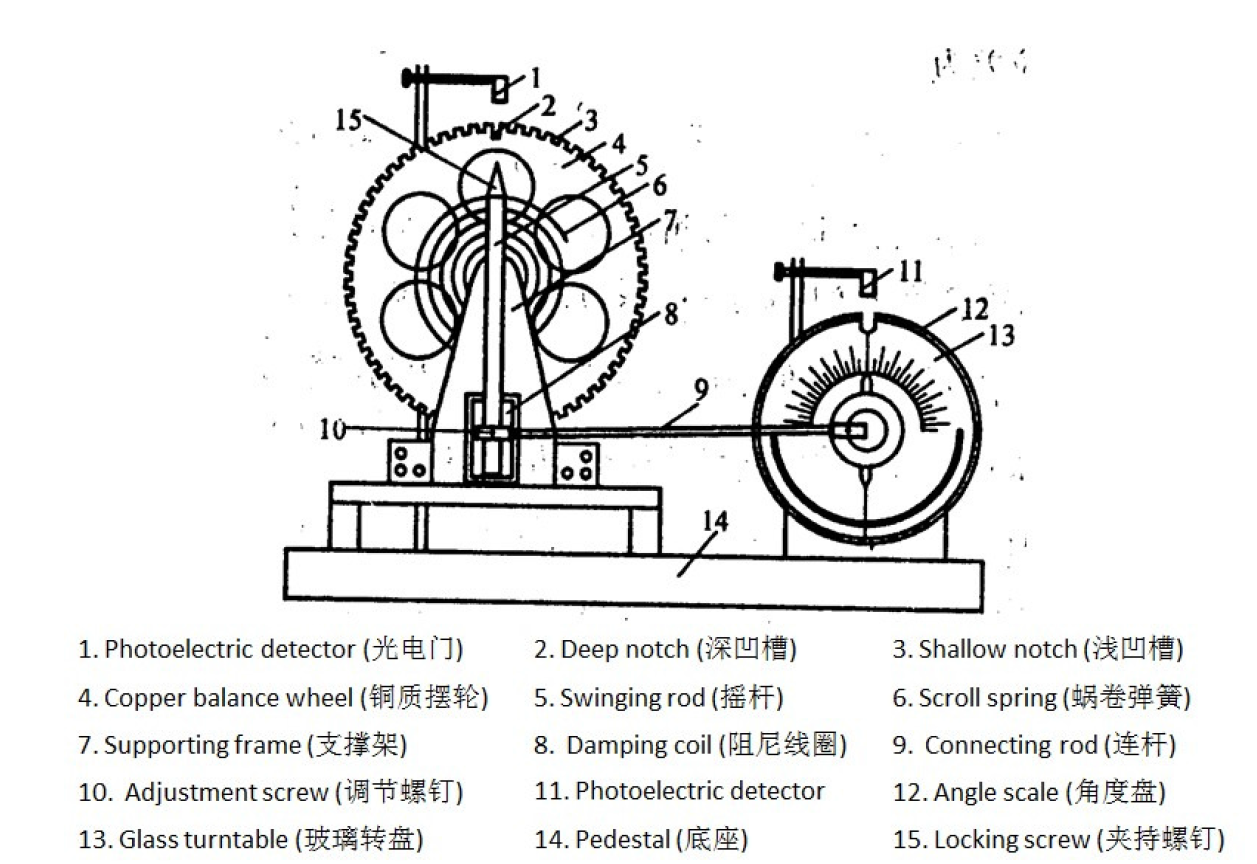
\includegraphics[scale=0.5]{P2.jpg}
\caption{Experiment Scheme}
\end{figure}
\par According to Fresnel equations, $$t=\frac{2n_i\cos\theta_i}{(n_i\cos\theta_i+n_t\cos\theta_t)}$$
so the transmission coefficient from light $t=\frac{2*1*\cos39.5^o}{1*\cos39.5^o+0}=2$
\section{PARTC: Diffraction}
\subsection{Measured Data}
The distance between the slit and screen is $35cm$. The distance between the 0 light center and 1 and -1 dark patterns is $0.5cm$. I guess the width of slit is less than or slightly larger than $632.8nm$. 
\subsection{Answers for Post Lab Questions}
According to $$y_m=x\frac{m\lambda}{a},a=x\frac{m\lambda}{y_m}=35*10^{-2}*\frac{632.8*10^{-9}}{1*10^{-2}}=0.22mm$$

\end{document}